\section{Associations}
\label{sec:classdiagrams-associations}

Classes may have associations to model relationships between the instances of the two classes involved in the association.
Associations elaborate data items (\code{Carrier Sets}, \code{Constants} and \code{Variables}) in the same way that Classes do, by setting an \code{Elaborates} link in the properties view.
The generated predicates for the association, depend on its cardinality which is controlled by four boolean fields, \code{surjective}, \code{injective}, \code{total} and \code{functional} in the property view.
These fields have the following meaning:
\begin{itemize}
	\item \code{surjective} - all instances of the target class have at least one value in the association. (True corresponds to min cardinality = 1 at the source end).
	\item \code{injective} - all instances of the target class have at most one value in the association. (True corresponds to max cardinality = 1 at the source end). 
	\item \code{total} - all instances of the source class have at least one value in the association. (True corresponds to min cardinality = 1 at the target end).
	\item \code{functional} - all instances of the source class have at most one value in the association. (True corresponds to max cardinality = 1 at the target end).
\end{itemize}

The generated predicates for each case are shown in Table~\ref{tab:AssociationMultiplicity}. The table also shows the corresponding association cardinalities as shown on the diagram. 
The default value is a relation (all false) which is the least constrained option.

%----------------------------------------------------------
%Cardinality controls for associations
%----------------------------------------------------------
\begin{table}[!htb]  
	\centering 
	\begin{tabular}{|l|l|l|l|l|l|l|} 
		\hline 
		\textbf{Card} &\textbf{Surj.} & \textbf{Inj.} & \textbf{Total} & \textbf{Func.} & \textbf{Generated predicates} & \textbf{Description}\\ 
		\hline 
		0..n - 0..n&false&false&false&false&$a \in{} S \rel{} T$&relation\\ 
		\hline 
		1..n - 0..n&true&false&false&false&$a \in{} S \srel{} T$&surjective relation\\ 
		\hline 
		0..1 - 0..n&false&true&false&false&$a \in{} S \rel{} T, ~~ a\converse{} \in{} S \pfun{} T$&converse function\\ 
		\hline 
		1..1 - 0..n&true&true&false&false&$a \in{} S \srel{} T,~~  a\converse{} \in{} S \pfun{} T$&surj. rel. and conv. fn\\ 
		\hline 
		0..n - 1..n&false&false&true&false&$a \in{} S \trel{} T$&total relation\\ 
		\hline 
		1..n - 1..n&true&false&true&false&$a \in{} S \strel{} T$&surjective total relation\\ 
		\hline 
		0..1 - 1..n&false&true&true&false&$a \in{} S \trel{} T,~~  a\converse{} \in{} S \pfun{} T$&total rel. and conv. fn.\\ 
		\hline 
		1..1 - 1..n&true&true&true&false&$a \in{} S \strel{} T,~~  a\converse{} \in{} S \pfun{} T$&surj. total rel. and conv. fn.\\ 
		\hline 
		0..n - 0..1&false&false&false&true&$a \in{} S \pfun{} T$&partial function\\ 
		\hline 
		1..n - 0..1&true&false&false&true&$a \in{} S \psur{} T$&partial surjection\\ 
		\hline 
		0..1 - 0..1&false&true&false&true&$a \in{} S \pinj{} T$&partial injection\\ 
		\hline 
		1..1 - 0..1&true&true&false&true&$a \in{} S \psur{} T,~~  a\converse{} \in{} S \pfun{} T$&partial surj. and conv. fn\\ 
		\hline 
		0..n - 1..1&false&false&true&true&$a \in{} S \tfun{} T$&total function\\ 
		\hline 
		1..n - 1..1&true&false&true&true&$a \in{} S \tsur{} T$&total surjection\\ 
		\hline 
		0..1 - 1..1&false&true&true&true&$a \in{} S \tinj{} T$&total injection\\ 
		\hline 
		1..1 - 1..1&true&true&true&true&$a \in{} S \tbij{} T$&total bijection\\ 
		\hline 
	\end{tabular} 
	\caption{Association multiplicity controls for an association \code{a} from class \code{S} to class \code{T}} 
	\label{tab:AssociationMultiplicity} 
\end{table} 

Fig.~\ref{fig:ClassAssociations} shows an example variable association \code{particles} from class \code{hadrons} to class \code{quarks}.
The example is injective because a quark can only belong to at most one hadron and total because all hadrons are made from particles, but it is not surjective because quarks can exist independently of hadrons and not functional because hadrons are composed of several quarks.
The Event-B for this example is shown below:
\MACHINE{Associations}{}{AssociationsContext}{}
\VARIABLES{
	\Variable{particles}{}
	\Variable{hadrons}{}
	\Variable{quarks}{}
}
\INVARIANTS{
	\Invariant{Quarks\_supertypeOf\_quarks}{false}{$quarks \in{} \pow{}(Quarks)$}{}
	\Invariant{Hadrons\_supertypeOf\_hadrons}{false}{$hadrons \in{} \pow{}(Hadrons)$}{}
	\Invariant{assocMult\_particles}{false}{$particles \in{} hadrons \trel{} quarks$}{}
	\Invariant{assocMultInjective\_particles}{false}{$particles\converse{} \in{} quarks\pfun{}hadrons$}{}
}
\EVENTS{
	\INITIALISATION{false}{}{
		\ACTIONS{false}{
			\Action{init\_quarks}{$quarks \bcmeq{} \emptyset{}$}{true}{}
			\Action{init\_hadrons}{$hadrons \bcmeq{} \emptyset{}$}{true}{}
			\Action{init\_particles}{$particles \bcmeq{} \emptyset{}$}{true}{}
		}
	}
}
\END

\emph{Note: There is an} \code{Initial Value} \emph{property field for associations, but this is rarely used. For variable associations, the value is normally decided by a creation method parameter and for constant associations it is usually desirable to leave the value underspecified for genericity.}

\begin{figure}[!htbp]
	\centering
	\ifplastex
	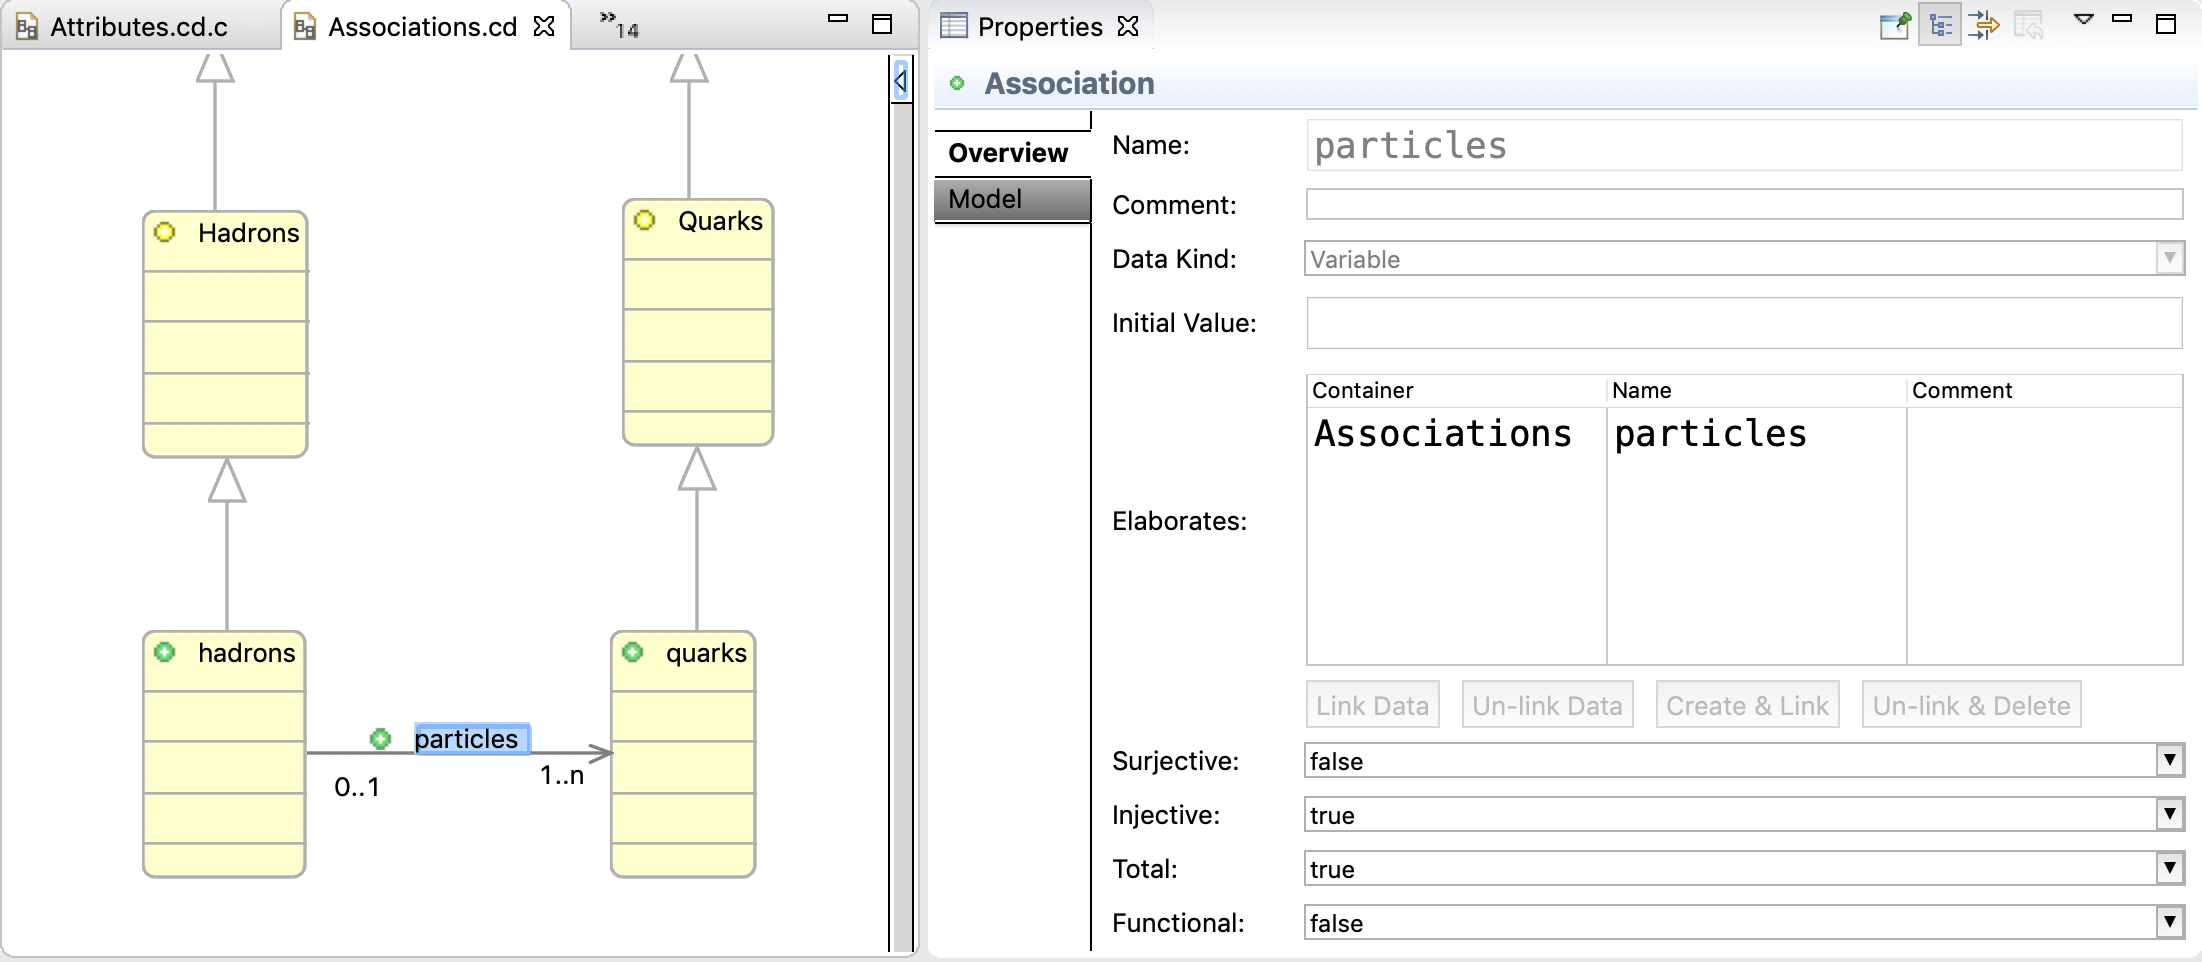
\includegraphics[width=1000]{figures/ClassAssociations.png}
	\else
	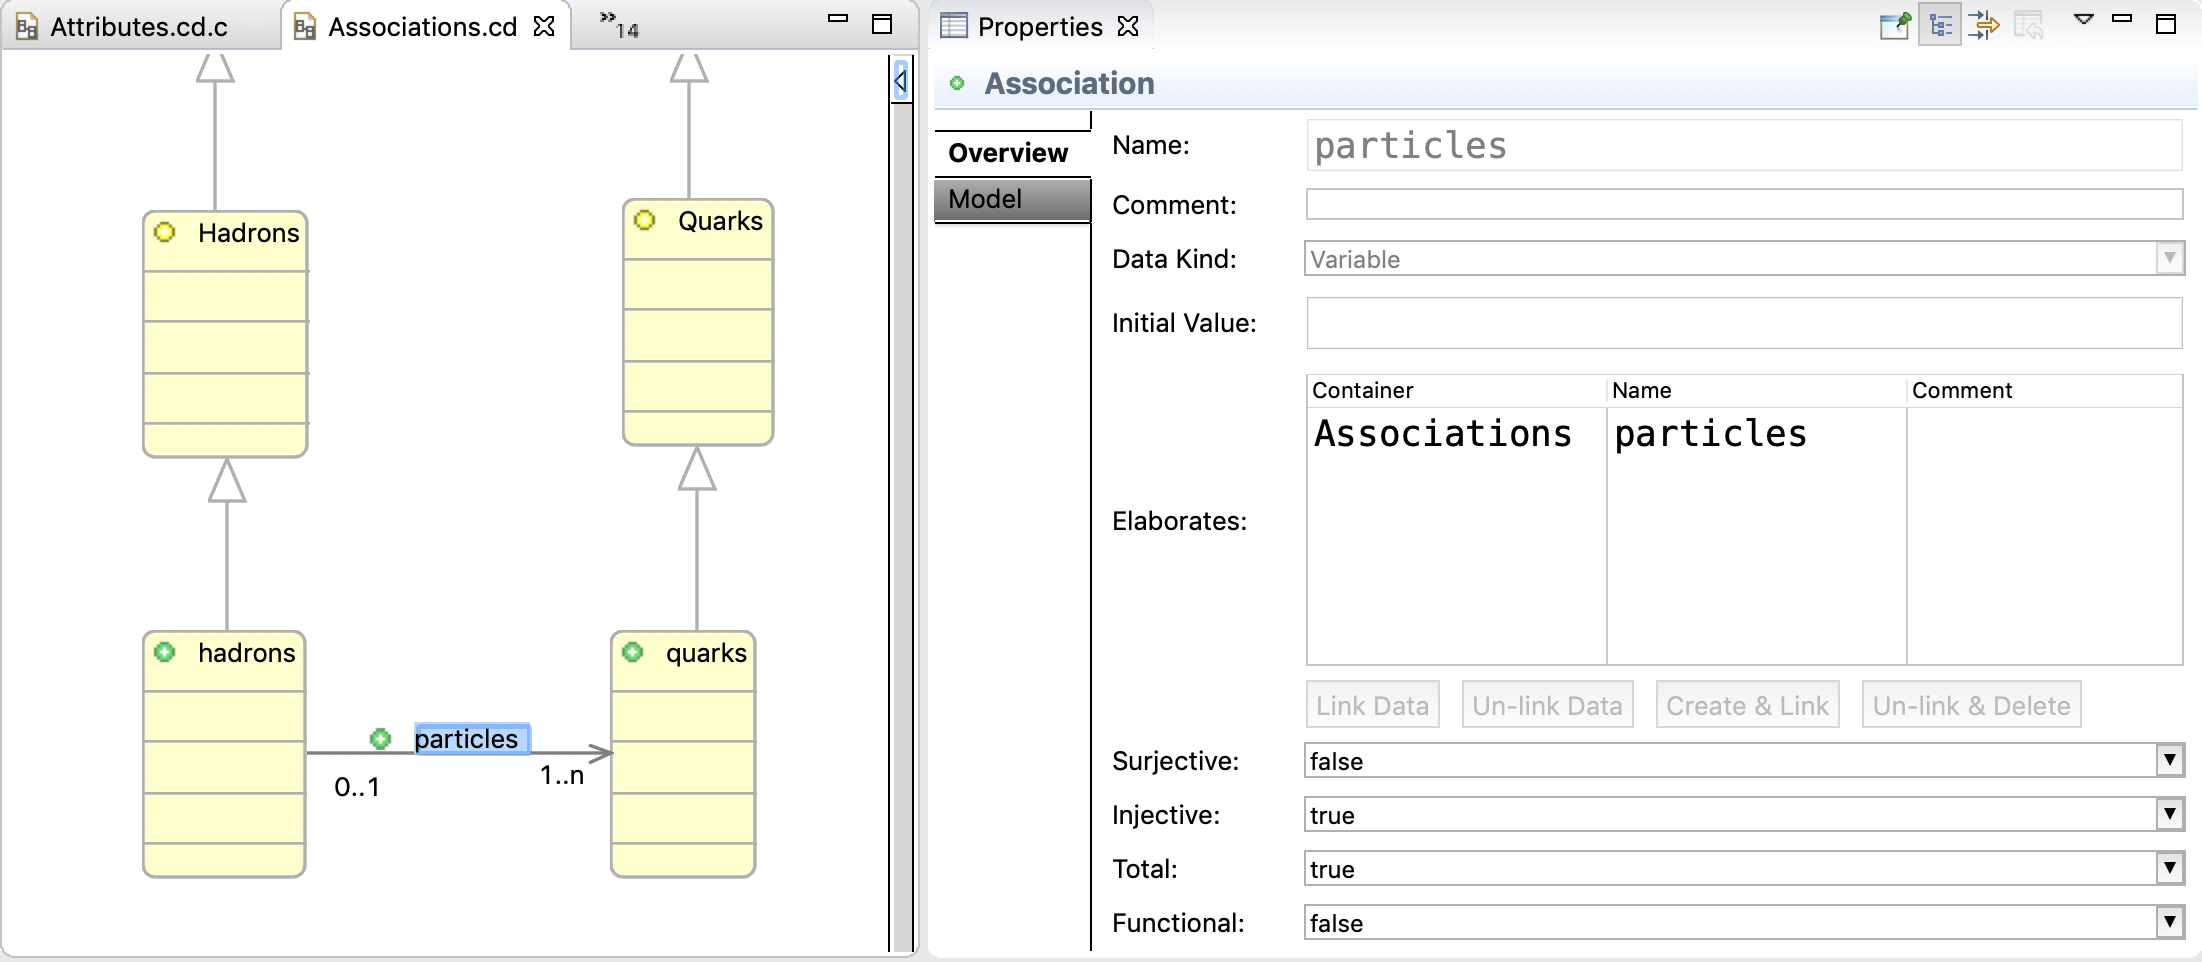
\includegraphics[width=1\textwidth]{figures/ClassAssociations.png}
	\fi
	\caption{An association between two classes}
	\label{fig:ClassAssociations}
\end{figure}